% Emacs settings: -*-mode: latex; TeX-master: "manual.tex"; -*-

\chapter{Samples}
\index{Library!Components!samples}

This class of components models the sample of the experiment.
This is by far the most challenging part of a neutron scattering
instrument to model. However, for purpose of simulating
instrument performance, details of the samples are rather unimportant,
allowing for simple approximations. On the contrary, for full
virtual experiments it is of importance to have realistic and
detailed sample descriptions. \MCS\ contains both simple and detailed
samples, although there is still room for much more development.

We first consider incoherent scattering. The simple component {\bf Vanadium}
performs both incoherent scattering and absorption.

An important component class is elastic Bragg scattering from an ideal powder.
The components {\bf Powder1} and {\bf Powder2} model a simple powder with one or two
reflections and incoherent scattering. Finally, the {\bf PowderN} component extends the capabilities to N lines, read from a LAZY/Crystallographica data file.

Next type is Bragg scattering from single crystals.
The simplest single crystals are in fact the monochromator components
{\bf Monochromator\_flat} and {\bf Monochromator\_curved},
which were presented in the section on optics.
The monochromators are models of a thin mosaic crystal
with a single scattering vector perpendicular to the surface.
Much more advanced, the component {\bf Single\_crystal}
is a general single crystal sample (with multiple scattering) that allows
the input of an arbitrary unit cell and a list of structure factors, and
also allows anisotropic mosaic and $\Delta d/d$ lattice space variation.

Isotropoic small-angle scattering is simulated in {\bf Sans\_Spheres},
which models scattering from a collection of hard spheres. A more general
SANS sample is highly wanted. In addition, a reflectometry sample
should be developed.

Inelastic scattering from a dispersion is exemplified by
the relatively simple component {\bf Phonon}.

For a more general sample model, the {\bf Isotropic\_Sqw} component is able to simulate all kinds of isotropic materials: liquids, glasses, polymers, powders, ... Physical processes include coherent/incoherent scattering, both elastic and inelastic, with absorption and multiple scattering. Moreover, this compoennt may be used concentrically, to model a sample environment. Thus it may handle most samples except single crystals.

In general, all samples are assumed to be homogeneous. There would also be
potential in developing an inhomogeneous sample, e.g. with
spatially varying lattice constant, relevant for stress/strain scanners.
Inhomogeneously absorbing sample for tomography could also be possible.
Further, no polarization effects are yet taken into account in any
of the samples.

\begin{table}
  \begin{center}
  {\let\my=\\
    \begin{tabular}{|c|cc|cc|c|c|}
    \hline
    Sample        & \multicolumn{2}{c|}{Coherent} & \multicolumn{2}{c|}{Incoherent} &&\\
    Process       & Elastic & Inelastic & Elastic & Inelastic & Absorption & Multi. Scatt.\\
    \hline
    Phonon\_simple&         & X         &         &           & X & \\
    Isotropic\_Sqw&  X      & X         & X       & X         & X & X \\
    Powder1       &  1 line &           &         &           & X & \\
    PowderN       &  N lines&           &         &           & X & \\
    Sans\_spheres &  colloid&           &         &           & X & \\
    Single\_crystal& X      &           & X       &           & X & X \\
    V\_sample     &         &           & X       &           & X & \\
    \hline
    \end{tabular}
    \caption{Processes implemented in sample components}
    \label{t:sample-process}
  }
  \end{center}
\end{table}

\input{vanadium.tex}
\input{powder2.tex}
\input{Single_crystal.tex}
\section{Sans\_spheres: A sample of hard spheres for small-angle scattering}
\label{sans}
\index{Samples!Dilute colloid medium}
\index{Diffraction}
\index{Small angle scattering}

\component{Sans\_spheres}{(System); Lise Arleth, Veterinary University of Denmark}{$R$, $x_w$, $y_h$, $z_t$, $r$, $\sigma_a$}{$phi$, $q_{max}$, $\Delta \rho$}{}

The component {\bf Sans\_spheres} models a sample of small independent
spheres of radius $R$, which are uniformly distributed
in a rectangular volume $x_w \times y_h \times z_t$ with a volume
fraction $\phi$. The absorption cross section density for the spheres
(or is it from the solution?)
is $\sigma_a$ (in units of m$^{-1}$), specified
for neutrons at 2200 m/s. Absorption and incoherent scattering from the medium
is neglected.
The difference in scattering length density
(the contrast) between the hard spheres and the medium is called $\Delta \rho$.
$q_{\rm max}$ denotes the maximum scattered $q$-value that is probed
in the simulation.

\subsection{Small-angle scattering cross section}
The neutron intensity scattered in a solid angle $\Delta \Omega$
for a flat transmission isotropic SANS sample is given by \cite{ILLblue}:
\begin{equation}
I_s(q) = \Psi \Delta\Omega T A z_{\rm max} \frac{d\sigma_v}{d\Omega}(q) ,
\end{equation}
where $\Psi$ is the neutron flux, $T$ is the sample transmission,
$A$ is the illuminated sample area, and $z_{\rm max}$ the length of
the neutron path through the sample.

In this component, we consider only scattering from a thin solution
of monodisperse hard spheres of radius $R$, where the volume-specific
scattering cross section is given by \cite{ILLblue}
\begin{equation}
\frac{d\sigma_v}{d\Omega}(q) =
  n (\Delta\rho)^2 V^2 \left( 3\frac{\sin(qR)-qR\cos(qR)}{(qR)^3} \right)^2 .
\end{equation}
Here, $n$ is the number density of spheres, and $V$ is the
sphere volume. Their product gives the input parameter, $\phi=nV$.

\subsection{Algorithm}
All neutrons, which hit the sample volume, are scattered.
(Hence, no direct beam is simulated.)
For scattred neutrons, the following steps are taken:
\begin{enumerate}
\item Choose a value of $q$ uniformly in the interval $[0;q_{\rm max}]$.
\item Choose a polar angle, $\alpha$,
  for the {\bf q}-vector uniformly in $[0;\pi]$.
\item Scatter the neutron according to $(q,\alpha)$.
\item Calculate and apply the correct weight factor correction.
\end{enumerate}

% Emacs settings: -*-mode: latex; TeX-master: "manual.tex"; -*-


\section{Phonon\_simple: A simple phonon sample}
\label{s:phonon_simple}
\index{Samples!Isotropic acoustic phonon}
\index{Inelastic scattering}

\component{Phonon\_simple}{Kim Lefmann}{ $r_{\rm o}$, $h$, $r_{\rm foc}$, $x_{\rm target}$, $y_{\rm target}$, $z_{\rm target}$, $\sigma_{\rm abs}$, $\sigma_{\rm inc}$, $a$, $b$, $M$, $c$, $DW$, $T$}{$w_x$, $h_y$, $t_z$, $w_{\rm focus}, h_{\rm focus}$, $w_{\rm foc, angle}$, $h_{\rm foc, angle}$, target\_index}{}
This component models a simple phonon signal from a single crystal of 
one element in an {\em fcc} crystal structure.
Only one isotropic acoustic phonon branch is modeled, and the longitudinal
and transverse dispersions are identical with the velocity of sound being $c$.
Other physical parameters are the atomic mass, $M$, the lattice parameter, $a$,
the scattering length, $b$,
the Debye-Waller factor, \verb+DW+, and the temperature, $T$.

Incoherent scattering and absorption are also taken into account by the cross
sections $\sigma_{\rm abs}$ and $\sigma_{\rm inc}$.

The sample can have the form of a cylinder with height $h$ and radius
$r_0$, or a box with dimensions $w_x, h_y, t_z$. 

Phonons are emitted into a specific range of solid angles, specified 
by the location $(x_t, y_t, z_t)$ and the focusing radius, $r_0$.
Alternatively, the focusing is given by a rectangle, 
$w_{\rm focus}$ and $h_{\rm focus}$, and the focus point is given by the
indeox of a down-stream optical element, \verb+target_index+.

Multiple scattering is not included in this component. The scattering
cross section is given by the detailed calculations below.

\subsubsection{The phonon cross section} % This is taken directly from the paper %
The inelastic phonon cross section for a Bravais crystal of a pure element
is given by Ref.~\cite[ch.3~]{squires} 
\begin{eqnarray}
\frac{d^2\sigma'}{d\Omega dE_{\rm f}} &=&
  b^2 \frac{k_{\rm f}}{k_{\rm i}} \frac{(2\pi)^3}{V_0}\frac{1}{2M} \exp(-2W) \nonumber \\
&\times&
  \sum_{\tau,q,p} \frac{(\mbox{\boldmath $\kappa$} \cdot {\bf e}_{q,p})^2}
                       {\omega_{q,p}} 
  \left\langle n_{q,p} + \frac{1}{2} \mp \frac{1}{2} \right\rangle
  \delta(\omega\pm\omega_{q,p}) \delta(\kappa\pm{\bf q}-\tau) ,
\end{eqnarray}
where both annihilation and creation of one phonon is considered
(represented by the plus and minus sign in the dispersion relation,
respectively).
In the equation, 
$\exp(-2W)$ is the Debye-Waller factor, \verb+DW+ and
$V_{\rm c} = \rho_{\rm c}^{-1}$ is the volume of the unit cell.
The sum runs over the reciprocal lattice vectors, $\tau$, 
over the polarisation index, $p$,
and the $N$ allowed wave vectors {\bf q} within the Brillouin zone
(where $N$ is the number of unit cells in the crystal).
Further, ${\bf e}_{q,p}$ is the
polarization unit vectors, $\omega_{q,p}$ the phonon dispersion,
and $\langle n_{q,p} \rangle$ is the Bose factor at the given value of
$\hbar |\omega_{q,p}|/(k_{\rm B}T)$.

We have simplified this expression by assuming no polarization
dependence of the dispersion, giving 
$\sum_{p} (\mbox{\boldmath $\kappa$} \cdot {\bf e}_{q,p})^2 = \kappa^2$.
We assume that the inter-atomic interaction is nearest-neighbour-only
so that the phonon dispersion becomes: 
\begin{equation}
d_1({\bf q}) = c_1/a \sqrt(z-s_q) ,
\end{equation}
where $z=12$ is the number of nearest neighbours and 
$s_q=\sum_{\rm nn} \cos({\bf q} \cdot {\bf r}_{\rm nn})$,
where in turn ${\bf r}_{\rm nn}$ is the lattice positions of the 
nearest neighbours.

This dispersion relation may be modified with a small effort,
since it is given as a separate c-function attatched to the component.

To calculate $d\sigma/d\Omega$ we need to transform the 
{\bf q} sum into an integral over the Brillouin zone by 
$\sum_q \rightarrow N V_{\rm c} (2\pi)^{-3} \int_{\rm BZ} d^3{\bf q}$.
The $\mbox{\boldmath $\kappa$}$ sum can now be removed by
expanding the {\bf q} integral to infinity. 
All in all, the partial differential cross section reads
\begin{eqnarray}
\frac{d^2\sigma'}{d\Omega dE_{\rm f}}
  (\mbox{\boldmath $\kappa$},\omega) &=&
  b^2 \frac{k_{\rm f}}{k_{\rm i}} N \frac{1}{2M} 
  \int \frac{\hbar \kappa^2}{c_1 |{\bf q}-{\bf Q}|} 
  \left\langle n_{q}+\frac{1}{2}\mp\frac{1}{2} \right\rangle
  \delta(\omega\pm\omega_{q}) \delta(\mbox{\boldmath $\kappa$}\pm{\bf q}) 
   d^3{\bf q} \nonumber \\
 &=& b^2 \frac{k_{\rm f}}{k_{\rm i}} N 
          \frac{\hbar^2 \kappa^2}{2M c_1|{\bf q}-{\bf Q}|} 
  \left\langle n_{\kappa}+\frac12\pm\frac12 \right\rangle 
  \delta(\hbar\omega\pm d_1(\kappa)) .
\end{eqnarray}
Using the integration sketched in eq.~(\ref{eq:dcsdisp}), we reach
*** CHECK THIS!! ***
\begin{equation} \label{eq:phononcross}
\left(\frac{d\sigma'}{d\Omega}\right)_j =
b^2 \frac{k_{\rm f}^2}{k_{\rm i}} N 
\frac{\hbar^4 \kappa^2}{2Mm c_1 |{\bf q}-{\bf Q}| J(k_{{\rm f},j})} 
\left\langle n_{\kappa}+\frac12\pm\frac12 \right\rangle . 
\end{equation}
A rough order-of-magnitude consideration gives
$\frac{\hbar^2 k_{{\rm f},j}}{mJ(k_{{\rm f},j})} \approx 1$,
$\frac{k_{{\rm f},j}}{k_{{\rm f},i}}\approx 1$,
$\langle n_{\kappa}+\frac12\pm\frac12 \rangle \approx 1$,
$\frac{\hbar^2\kappa^2}{2M\hbar\omega_\kappa}
\approx \frac{m}{M}$ (for large disperison values?????).
Hence, $\left(\frac{d\sigma}{d\Omega}\right)_j \approx N b^2 \frac{m}{M}$, and
$\sigma_{\rm inel}$ becomes a fraction of $4 \pi N b^2$, as one
would expect.
The differential cross section per unit cell is found from 
(\ref{eq:phononcross}) by letting $N=1$. 

\subsubsection{The algorithm}
(*** SEE IF THIS IS WRITTEN ELSEWHERE ***)

\subsubsection{The weight transformation}
The total weight transformation becomes
\begin{equation} \label{eq:phonon_mult}
\pi_i = a_{\rm lin} \rho_c l_{\rm max} n_{\rm s} \Delta \Omega
 b^2 \frac{k_{\rm f}^2}{k_{\rm i}}
 \frac{\hbar^4 \kappa}{2Mm c_1 |{\bf q}-{\bf Q}| J(k_{{\rm f},j})} 
 \left\langle n_{\kappa}+\frac12\pm\frac12 \right\rangle ,
\end{equation}
where the Jacobian reads
\begin{equation}
J = -\frac{\hbar^2}{m} k_{\rm f} 
    - c \frac{\partial}{\partial k_{\rm f}} 
        \left| {\bf k}_{\rm i} - k_{\rm f} \hat{k}_{\rm f} \right| .
\end{equation}



\section{Isotropic\_Sqw: A general $S(q,\omega)$ coherent and incoherent scatterer}
\label{s:isotropic-sqw}
\index{Samples!Coherent and incoherent isotropic scatterer}
\index{Coherent and incoherent isotropic scatterer}
\index{Inelastic scattering}

\component{Isotropic\_Sqw}{V. Hugouvieux, E. Farhi}{Sqw$\_{coh}$, $\sigma_{coh}$, Sqw$\_{inc}$, $\sigma_{inc}, V_\rho, \sigma_{abs}, T$}{$q_{min}, q_{max}, \omega_{min}, \omega_{max}, d\phi$, order}{not fully validated}

\begin{figure}
  \begin{center}
    \includegraphics[width=0.9\textwidth]{figures/sqw.eps}
  \end{center}
\caption{An $l-^4$He sample in a cryostat, simulated with the Isotropic\_Sqw component in concentric geometry.}
\label{f:isotropic-sqw}
\end{figure}

The component assumes that the sample has the structure of a liquid. This stands for indeed normal liquids, glasses (amorphous systems), polymers, and may be extended to powders.

\subsection{A short introduction to the theory of liquids}

\begin{figure}
  \begin{center}
    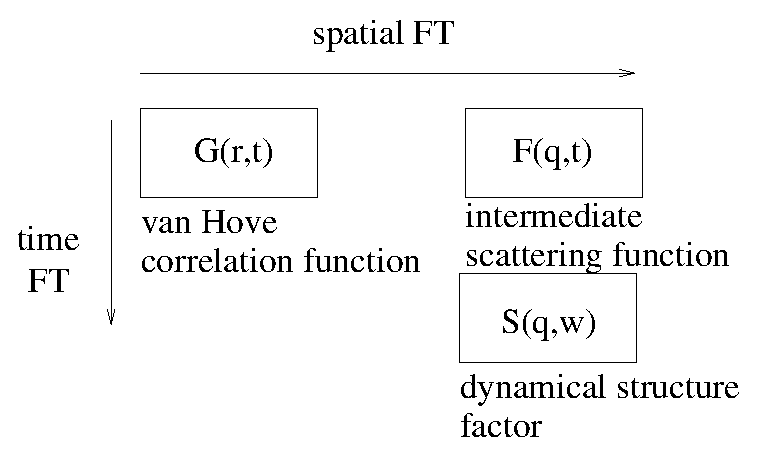
\includegraphics[width=0.9\textwidth]{figures/GFS.eps}
  \end{center}
\caption{Relations between dynamical functions using space, time, wavevector and energy variables.}
\label{f:GFS}
\end{figure}

In the case of a homogeneous and classical liquid, the \emph{van Hove correlation function}, which describes the time and space correlations in the liquid, can be written \cite{Egelstaff67,squires}:
\begin{equation} \label{eq:vanhove}
G(\vec{r},t) = \frac{1}{N} \sum_{i=1}^N \sum_{j=1}^N  \langle\delta[\vec{r} + \vec{r}_i(0) - \vec{r}_j(t)]\rangle
\end{equation}
with $\vec(r)$ and $t$ being the position and time of the atom distribution in the liquid.
Using the particule-density function $\rho(\vec(r),t)$, the function $G$ can be rewritten:
\begin{equation} \label{eq:vanhove-rho}
G(\vec{r},t) = \frac{\langle \rho(0,0) \rho(\vec{r},t)\rangle}{\rho}
\end{equation}

On the experimental point of view, one usually refers to the \emph{dynamical structure factor} $S(q,\omega)$, which is the double Fourier-transform in space and time of the van Hove correlation function $G(r,t)$:
\begin{eqnarray} \label{eq:sqw-rho}
S(q,\omega) &= \frac{1}{2\pi}\int_{-\infty}^{\infty} F(\vec{q},t) e^{-i\omega t} dt \nonumber \\
            &= \frac{1}{2\pi N} \int_{-\infty}^{\infty} \langle \hat\rho^*(\vec{q},0) \hat\rho(\vec{q},t) \rangle e^{-i\omega t} dt.
\end{eqnarray}
where $\hat\rho(\vec{q}, t)$ is the spatial Fourier transform of the density $\rho(\vec{r},t)$, and the \emph{intermediate scattering function} $F$ is the time correlation function of $\hat\rho$:
\begin{eqnarray}
F(\vec{q},t) &= \frac{1}{N} \langle \hat\rho^*(\vec{q},0)  \hat\rho(\vec{q},t) \rangle \nonumber \\
                    &= \frac{1}{N} \sum_{i=1}^N \sum_{j=1}^N \langle e^{i \vec{q}.(\vec{r}_j(t) - \vec{r}_i(0))} \rangle
\end{eqnarray}
Some easely measureable quantities in a liquid are the \emph{pair correlation function} $g(r)$ and the \emph{structure factor} $S(q)$, defined as:
\begin{eqnarray}
\rho g(\vec{r}) &= \frac{1}{N} \sum_{i=1}^N \sum_{j \neq i} \langle \delta(\vec{r}+\vec{r}_i-\vec{r}_j) \rangle \\
S(\vec{q}) &=1 + \rho \int_V [g(\vec{r})-1] e^{i\vec{q}.\vec{r}} d\vec{r} \\
           &=1 + \rho \int_{0}^{\infty} [g(r)-1] \frac{\sin(qr)}{qr} 4 \pi r^2 dr {\rm in isotropic materials}
\end{eqnarray}
Both $g(r)$ and $S(q)$ converge to unity for large $r$ and $q$ values respectively, and they are representative of the atoms spatial distribution.


Following Squires (\cite{squires}, p63), the neutron differential scattering cross section for both coherent and incoherent processes is
\begin{equation}
\frac{d^2\sigma}{d\Omega dE_f} = \frac{\sigma}{4\pi}\frac{k_f}{k_i} N S(q, \omega)
\end{equation}
with usual notations. The unit of the dynamical structure factor $S$ is an inverse energy.

\subsection{How does a neutron interact with the material ?}


\subsection{The implementation}
\subsubsection{Choosing the interaction position}
\subsubsection{Choosing the type of interaction}
\subsubsection{Choosing the $q$ and $\omega$ transfert}
%\input{LSCO.tex}

